\chapter{Les anti-patrons dans les APIs RESTful}
L’architecture SOA est devenue une parmi les plus architecutre adoptées,surtout son style architectural «REpresentational State Transfer» privilégié par beaucoup d’entreprises de production de logiciels comme twitter, facebook et youtube.
Vu que les développeurs utilisant ces APIs ont besoins de les comprendre pour pouvoir les exploiter dans leurs applications web, c’est pourquoi, les développeurs tendent vers chercher les APIs dont les URIs (Uniform Resource Identifiers) sont bien conçus et bien \textbf{nommés}.

Les cinq anti-patrons linguistiques  apparus dans les applications REST \cite{palma2015restful}:
\begin{enumerate}
    

\item \textbf{Noms de ressources contextualisés vs Noms de ressources non-contextualisés}
\begin{itemize}
    

\item {Description}: l’URI doit être contextuel,ie, les nœuds d’une URI doivent être sémantiquement reliés au même contexte.Cet anti-patron apparaît si les nœuds d’une URI n’appartient pas sémantiquement au même contexte.
\item Exemple: \\
https://www.example.com/newspapers/players?id=123  est faux mais \\
https://www.example.com/newspapers/media/page?id=123 est correct.
\item Conséquences:\\
Les noms des ressources non-contextualisés ne fournissent pas un contexte clair pour les requêtes qui dégrade la compréhension des URIs de la part des développeurs qui les utilisent.
\end{itemize}

\item \textbf{Noeuds hiérarchiques vs nœuds non-hiérarchiques}
\begin{itemize}
    

\item Description: chaque nœud composant d’une URI doit être hiérarchiquement relié aux nœuds voisins, donc cet anti-patrons apparaît si on trouve des nœuds dans une URI qui ne sont pas hiérarchiquement reliés  à leurs nœuds voisins.
\item Exemple:\\
https://www.example.com/professors/university/faculty/ est faux mais\\ https://www.example.com/university/faculty/professors/ est correct.
\item Conséquences: ça peur induire à une confusion à propos de l’utilité de l’URI et donc son utilisabilité.
\end{itemize}
\item \textbf{URI propre vs URI amorphe}
\begin{itemize}
    

\item Description: Une URI propre est une URI lisible,dont les noms sont minuscules, sans underscore, sans extensions et sans aucun symbole pouvant compliquer la lecture de l’URI sinon cet anti-patron est identifié.
\item Exemple:\\
https://w\itemww.example.com/NEW Customer/ photo01.jpg/ est faux mais \\
https://www.example.com/customers/1234 est correct.
\item Conséquences: Les mots en lettres majuscules et en lettres minuscules ne signifient pas la même ressource,et en général ça peut mener vers une ambiguïté dans l'écriture de la requête.
\end{itemize}
\item \textbf{URI sans verbes vs une URI CRUDy}
\begin{itemize}
    

\item Description: Cet anti-patrons apparaît si les méthodes HTTPs : GET, PUT, POST,DELETE sont utilisés dans des URIs contenant des verbes comme create, update..etc
\item exemple:\\
POST https://www.example.com/update/players/age?id=123 est faux\\
mais POST https://www.example.com/players/age?id=123 est correct.
\item Conséquences:
Cet anti-patron cause une confusion, l’utilisateur d’une API risque de surcharger les méthodes http existantes.
\end{itemize}
\item \textbf{Noeuds singularisés vs Noeuds pluralisés}
\begin{itemize}
    

\item Description: Cet anti-patron apparaît si dans les requêtes put/delete, le dernier est au pluriel ou si dans les requêtes post le dernier nœud est au singulier
\item Exemple:\\
DELETE https://www.example.com/team/players \\
 POST https://www.example.com/team/player sont faux mais \\
DELETE https://www.example.com/team/player \\
 POST https://www.example.com/team/players sont corrects.
\item Conséquences:
Si un nœud pluriel est utilisé à la fin d’une URI de requête PUT/DELETE, le client de l’API ne peut pas créer/supprimer une collection de ressources qui peut causer la reponse serveur « 403 forbidden » et même si la réponse est filtrée,le client de l’API peut tomber dans la confusion entre est ce que le contenu accessible/supprimé est une ressource ou plusieurs ressources.
\end{itemize}
\end{enumerate}
La figure ci-dessous \ref{fig:algocontextualise} illustre l’algorithme de détection de l’anti-patrons « noms de ressources non-contextualisé» dans les applications RESTful \cite{palma2015restful}:
\begin{figure}[H]
	\centering
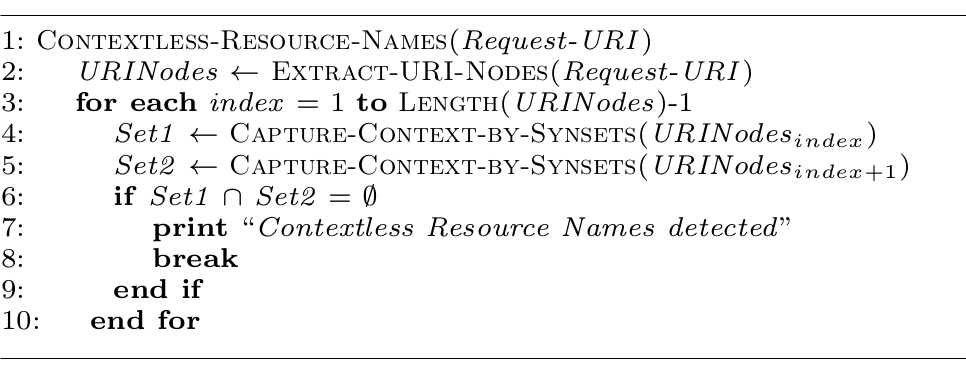
\includegraphics[width=0.9\linewidth]{Others/Resources/algocontextualis.png}
	\caption{L'algorithme de détection de l'anti-patron linguistique noms de ressources non contextualisés \cite{{arnaoudova2013new}}.}
		\label{fig:algocontextualise}
	\end{figure}

L’algorithme procède comme suit :
\begin{itemize}
\item On compare chaque pair de nœud dans une URI 
\item Si on trouve au moins une relation de non-contextualisation
\item Alors l’anti-patron de nom de ressources non-contextualisé.
\end{itemize}
L’ontology WordNet et Stanford CoreNLP pour capter les contextes et effectuer l’analyse sémantique \cite{palma2015restful}.
\\
\cite{palma2015restful} implémentent une solution qui s'appelle "DOLAR"(voir la figure \ref{dolar}) qui détecte les anti-patrons linguistiques dans les applications RESTful, l'article contient les détails de l'implémention ainsi que les résultats de ses tests.
\begin{figure}[H]
	\centering
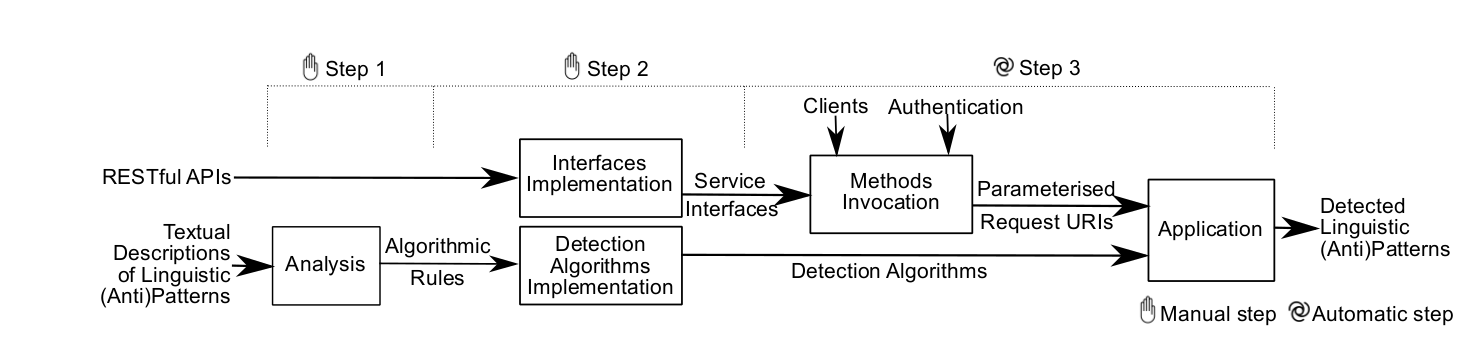
\includegraphics[width=\linewidth,length=10cm]{Others/Resources/dolarapproach.png}
	\caption{L'approche DOLAR \cite{{arnaoudova2013new}}.}
		\label{fig:dolar}
	\end{figure}
\vspace{5px}
\textbf{Conclusion:}
\newline
Le domaine d'anti-patrons linguistiques dans l'architecture SOA est un nouveau domaine, il n'est pas bien exploité, en observant le peu de travaux de recherches consacrés et les outils implémentés, ce qui nous encourage à plus chercher dans ce domaine et proposer des outils d'auto-refactoring.